\chapter{Evaluation}

To measure the effectiveness of dynamic windowing for multi-stream operators during the 
mapping of non-RDF heterogeneous data, we would need to measure the following 
metrics of our stream processing framework: \emph{latency}, \emph{throughput},
\emph{memory usage} and \emph{completeness}. \emph{Throughput}, in this 
paper, refers to the number of output/processed records per time unit. 
\emph{Latency, throughput,} and \emph{memory usage} can be measured following the recent benchmark studies by 
Van Dongen and Van den Poel(2020)~\cite{evalution_of_spe}.
However, to evaluate 
for the \emph{completeness/quality} of the generated output, a reference output needs 
to be generated for comparison. Since a data stream is in principle unbounded in nature, 
and cannot be processed completely to check for \emph{completeness}, a bounded 
dataset of relatively large volume could be used for \emph{completeness} measure.
To ensure consistency in the complexity of the multi-stream operator being used, 
we will apply the join operator in the windows --- a common operator used in 
data enrichment scenarios. 


The following sections will describe the methodology and the data used to evaluate the
different metrics. Setups required to reproduce the evaluation will also be elaborated 
in their respective sections. 


\section{Data}

Assessment of our dynamic windowing scheme for multi-stream operator will require 
the data to have some common attributes to enrich the data. Furthermore, to 
mirror the real-world scenario, we would also employ data gathered from IoT sensors
because of its common usage in data stream processing. We will use the same data 
as is the case for the benchmark in the paper by Van Dongen and Van den Poel~\cite{evalution_of_spe}. 
To recap, the data is provided by NDW (Nationale Databank Wegverkeersgegevens) from the 
Netherlands. It consists of measurements of the number of cars and their average speed. 
A subset of the complete sensor data will be replayed by a Kafka publisher into the two topics 
\emph{flow} and \emph{speed}, for the number of cars and the average speed respectively. 

\subsection{Data for completeness evaluation}
Completeness measure requires a dataset which could be mapped completely by a static 
mapping engine. RMLMapper \todo{maybe RMLStreamer for static set might be enough?} will
be used to generate our \emph{complete} output triples. Streaming data is usually 
ordered according to the event time and the same entity could appear in the 
stream at a different timestamp. This can lead to duplicates in the generated output by 
the RMLMapper. Therefore, duplicates in the generated output by the reference optimal
mapping engine needs to be removed in the final \emph{complete} output dataset.

\section{Evaluation pipeline}

\begin{figure}[!htbp]
    \centering
    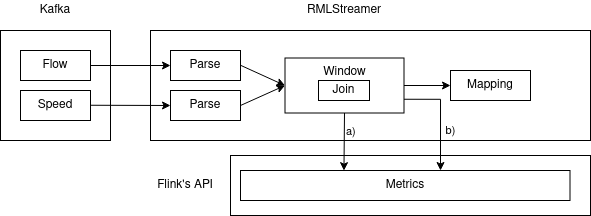
\includegraphics[width=\textwidth]{fig/evaluation_architecture.png}
    \caption{Evaluation flow based on~\cite{evalution_of_spe} with some changes to only 
    take metrics at the "Join" and the "Mapping" stage. a) \emph{throughput} of the generated output triple. 
    b) \emph{latency} of evaluating the join operator in windows.}
    \label{fig:evaluation_flow}
    
\end{figure}

Similar to the workflow process in~\cite{evalution_of_spe, benchmark_dsp}, we set up
our evaluation pipeline as illustrated in Figure~\ref{fig:evaluation_flow}. Setting it 
up according to the illustrated pipeline, allows us to have fine control over the 
workload scenarios and limit the measurement of the metrics just to the windows. 



\section{Workload scenarios}
As stated in Chapter~\ref{chap:data_stream_processing}, data streams have characteristics 
which determines the performance of stream processing frameworks and its operators. Therefore, 
there is a need to evaluate our dynamic window implementation under different workload scenarios. 

\subsection{Workload for maximum throughput measurement}
This workload will attempt to measure the maximum throughput RMLStreamer can 
process with the different windows, before \emph{latency,} and \emph{memory utilization}
increasing significantly. We will increase the velocity of the input data gradually 
every 10 seconds until there is a significant latency of more than 10 seconds to produce
the next output triple or until the memory allocated to the instances get fully used up. 


\subsection{Workload for latency measurement}



\subsection{Workload for failure restart}


\subsection{Workload for completeness}

\subsection{Workload with increasing burst }

\subsection{Workload with periodic burst}


\section{Environment}




